\documentclass{article}

% packages
  % basic stuff for rendering math
  \usepackage[letterpaper, top=1in, bottom=1in, left=1in, right=1in]{geometry}
  \usepackage[utf8]{inputenc}
  \usepackage[english]{babel}
  \usepackage{amsmath} 
  \usepackage{amssymb}
  % \usepackage{amsthm}

  % extra math symbols and utilities
  \usepackage{mathtools}        % for extra stuff like \coloneqq
  \usepackage{mathrsfs}         % for extra stuff like \mathsrc{}
  \usepackage{centernot}        % for the centernot arrow 
  \usepackage{bm}               % for better boldsymbol/mathbf 
  \usepackage{enumitem}         % better control over enumerate, itemize
  \usepackage{hyperref}         % for hypertext linking
  \usepackage{fancyvrb}          % for better verbatim environments
  \usepackage{newverbs}         % for texttt{}
  \usepackage{xcolor}           % for colored text 
  \usepackage{listings}         % to include code
  \usepackage{lstautogobble}    % helper package for code
  \usepackage{parcolumns}       % for side by side columns for two column code
  

  % page layout
  \usepackage{fancyhdr}         % for headers and footers 
  \usepackage{lastpage}         % to include last page number in footer 
  \usepackage{parskip}          % for no indentation and space between paragraphs    
  \usepackage[T1]{fontenc}      % to include \textbackslash
  \usepackage{footnote}
  \usepackage{etoolbox}

  % for custom environments
  \usepackage{tcolorbox}        % for better colored boxes in custom environments
  \tcbuselibrary{breakable}     % to allow tcolorboxes to break across pages

  % figures
  \usepackage{pgfplots}
  \pgfplotsset{compat=1.18}
  \usepackage{float}            % for [H] figure placement
  \usepackage{tikz}
  \usepackage{tikz-cd}
  \usepackage{circuitikz}
  \usetikzlibrary{arrows}
  \usetikzlibrary{positioning}
  \usetikzlibrary{calc}
  \usepackage{graphicx}
  \usepackage{caption} 
  \usepackage{subcaption}
  \captionsetup{font=small}

  % for tabular stuff 
  \usepackage{dcolumn}

  \usepackage[nottoc]{tocbibind}
  \pdfsuppresswarningpagegroup=1
  \hfuzz=5.002pt                % ignore overfull hbox badness warnings below this limit

% New and replaced operators
  \DeclareMathOperator{\Tr}{Tr}
  \DeclareMathOperator{\Sym}{Sym}
  \DeclareMathOperator{\Span}{span}
  \DeclareMathOperator{\std}{std}
  \DeclareMathOperator{\Cov}{Cov}
  \DeclareMathOperator{\Var}{Var}
  \DeclareMathOperator{\Corr}{Corr}
  \DeclareMathOperator{\pos}{pos}
  \DeclareMathOperator*{\argmin}{\arg\!\min}
  \DeclareMathOperator*{\argmax}{\arg\!\max}
  \newcommand{\ket}[1]{\ensuremath{\left|#1\right\rangle}}
  \newcommand{\bra}[1]{\ensuremath{\left\langle#1\right|}}
  \newcommand{\braket}[2]{\langle #1 | #2 \rangle}
  \newcommand{\qed}{\hfill$\blacksquare$}     % I like QED squares to be black

% Custom Environments
  \newtcolorbox[auto counter, number within=section]{question}[1][]
  {
    colframe = orange!25,
    colback  = orange!10,
    coltitle = orange!20!black,  
    breakable, 
    title = \textbf{Question \thetcbcounter ~(#1)}
  }

  \newtcolorbox[auto counter, number within=section]{exercise}[1][]
  {
    colframe = teal!25,
    colback  = teal!10,
    coltitle = teal!20!black,  
    breakable, 
    title = \textbf{Exercise \thetcbcounter ~(#1)}
  }
  \newtcolorbox[auto counter, number within=section]{solution}[1][]
  {
    colframe = violet!25,
    colback  = violet!10,
    coltitle = violet!20!black,  
    breakable, 
    title = \textbf{Solution \thetcbcounter}
  }
  \newtcolorbox[auto counter, number within=section]{lemma}[1][]
  {
    colframe = red!25,
    colback  = red!10,
    coltitle = red!20!black,  
    breakable, 
    title = \textbf{Lemma \thetcbcounter ~(#1)}
  }
  \newtcolorbox[auto counter, number within=section]{theorem}[1][]
  {
    colframe = red!25,
    colback  = red!10,
    coltitle = red!20!black,  
    breakable, 
    title = \textbf{Theorem \thetcbcounter ~(#1)}
  } 
  \newtcolorbox[auto counter, number within=section]{proposition}[1][]
  {
    colframe = red!25,
    colback  = red!10,
    coltitle = red!20!black,  
    breakable, 
    title = \textbf{Proposition \thetcbcounter ~(#1)}
  } 
  \newtcolorbox[auto counter, number within=section]{corollary}[1][]
  {
    colframe = red!25,
    colback  = red!10,
    coltitle = red!20!black,  
    breakable, 
    title = \textbf{Corollary \thetcbcounter ~(#1)}
  } 
  \newtcolorbox[auto counter, number within=section]{proof}[1][]
  {
    colframe = orange!25,
    colback  = orange!10,
    coltitle = orange!20!black,  
    breakable, 
    title = \textbf{Proof. }
  } 
  \newtcolorbox[auto counter, number within=section]{definition}[1][]
  {
    colframe = yellow!25,
    colback  = yellow!10,
    coltitle = yellow!20!black,  
    breakable, 
    title = \textbf{Definition \thetcbcounter ~(#1)}
  } 
  \newtcolorbox[auto counter, number within=section]{example}[1][]
  {
    colframe = blue!25,
    colback  = blue!10,
    coltitle = blue!20!black,  
    breakable, 
    title = \textbf{Example \thetcbcounter ~(#1)}
  } 
  \newtcolorbox[auto counter, number within=section]{code}[1][]
  {
    colframe = green!25,
    colback  = green!10,
    coltitle = green!20!black,  
    breakable, 
    title = \textbf{Code \thetcbcounter ~(#1)}
  } 

  \BeforeBeginEnvironment{example}{\savenotes}
  \AfterEndEnvironment{example}{\spewnotes}
  \BeforeBeginEnvironment{lemma}{\savenotes}
  \AfterEndEnvironment{lemma}{\spewnotes}
  \BeforeBeginEnvironment{theorem}{\savenotes}
  \AfterEndEnvironment{theorem}{\spewnotes}
  \BeforeBeginEnvironment{corollary}{\savenotes}
  \AfterEndEnvironment{corollary}{\spewnotes}
  \BeforeBeginEnvironment{proposition}{\savenotes}
  \AfterEndEnvironment{proposition}{\spewnotes}
  \BeforeBeginEnvironment{definition}{\savenotes}
  \AfterEndEnvironment{definition}{\spewnotes}
  \BeforeBeginEnvironment{exercise}{\savenotes}
  \AfterEndEnvironment{exercise}{\spewnotes}
  \BeforeBeginEnvironment{proof}{\savenotes}
  \AfterEndEnvironment{proof}{\spewnotes}
  \BeforeBeginEnvironment{solution}{\savenotes}
  \AfterEndEnvironment{solution}{\spewnotes}
  \BeforeBeginEnvironment{question}{\savenotes}
  \AfterEndEnvironment{question}{\spewnotes}
  \BeforeBeginEnvironment{code}{\savenotes}
  \AfterEndEnvironment{code}{\spewnotes}

  \definecolor{dkgreen}{rgb}{0,0.6,0}
  \definecolor{gray}{rgb}{0.5,0.5,0.5}
  \definecolor{mauve}{rgb}{0.58,0,0.82}
  \definecolor{lightgray}{gray}{0.93}

  % default options for listings (for code)
  \lstset{
    autogobble,
    frame=ltbr,
    language=C,                           % the language of the code
    aboveskip=3mm,
    belowskip=3mm,
    showstringspaces=false,
    columns=fullflexible,
    keepspaces=true,
    basicstyle={\small\ttfamily},
    numbers=left,
    firstnumber=1,                        % start line number at 1
    numberstyle=\tiny\color{gray},
    keywordstyle=\color{blue},
    commentstyle=\color{dkgreen},
    stringstyle=\color{mauve},
    backgroundcolor=\color{lightgray}, 
    breaklines=true,                      % break lines
    breakatwhitespace=true,
    tabsize=3, 
    xleftmargin=2em, 
    framexleftmargin=1.5em, 
    stepnumber=1
  }

% Page style
  \pagestyle{fancy}
  \fancyhead[L]{Macroeconomics}
  \fancyhead[C]{Muchang Bahng}
  \fancyhead[R]{Summer 2024} 
  \fancyfoot[C]{\thepage / \pageref{LastPage}}
  \renewcommand{\footrulewidth}{0.4pt}          % the footer line should be 0.4pt wide
  \renewcommand{\thispagestyle}[1]{}  % needed to include headers in title page

\begin{document}

\title{Macroeconomics}
\author{Muchang Bahng}
\date{Summer 2024}

\maketitle
\tableofcontents
\pagebreak

\section{Banks and Interest Rates}

  The entire economy comes from the role of banks and the interest rates (whatever that is) that is set upon them. There are many types of banks and many types of interest rates, which we will clarify. In any nation (we will use the U.S. as our primary example), we can divide all banks into the central bank and non-central banks. 
  \begin{enumerate}
    \item The Central Bank, known in the U.S. as the Federal Reserve. 
    \item Every other bank are their own identity. 
  \end{enumerate}
  The main difference between the central bank and other banks is that the central bank is \textit{not} a business, while the other banks are businesses, meaning that their purpose is the make money. The central bank's job is to control the economy and to prevent financial crises with the extra power they have as a part of the government (e.g. printing unlimited money, changing various rates). 

  There are multiple types of banks, mainly regarded with the audience they serve, ranging from individuals to small businesses to large conglomerates. We list the types of financial services they provide, but all of these activities boil down to the following: banks take the money that their customers deposit and invest them in other things for returns that are higher than the interest rates they give to the depositors. 
  \begin{enumerate}
    \item Retail banking provides financial services to the general public, allowing consumers to manage their money by giving them access to basic banking services, credit, and financial advice. These can be through checkings/savings accounts, CDs, safe deposit boxes, mortgages, and auto loans. 
    \item Commercial/corporate banking serves businesses ranging from small/mid-sized local businesses to large conglomerates. Corporate banking is a key profit center for most banks. 
    \item Investment banking provides financial services to companies within large and complex financial transactions. They focus mainly on company valuation to prepare for underwriting, M\&A, IPOs, and corporate reorganization. and they can be thought of as financial middlemen. 
  \end{enumerate}

  The separation between commercial and investment banking has been one of the primary features of the U.S. financial system since the 1930s. Congress is responsible for this separation, having decided that the investment banking activities of the nation's large commercial banks contributed to the widespread bank failures of the Depression. To prevent further failures, it passed legislation in 1935 called the Glass-Steagall Act that created a wall between commercial and investment banking activities and authorized a federal deposit insurance (FDIC) system. Investment banking, which involves dealings in stocks and bonds, was considered both risky and unsound for commercial banks that collected savings from the public.

  Since the Depression, a number of academic studies have suggested that such investment banking activities did not significantly contribute to massive bank failures. In addition, many now argue that the U.S. commercial banking system would actually be stronger if banking organizations were permitted to affiliate directly with investment banking concerns, a system usually referred to as universal banking. It turns out that the only major nations that require this is the U.S. and Japan, which was required to adopt this system after World War 2. Other large industrial countries like Germany and Switzerland have universal banking. The Glass-Steagall act was largely repealed in 1999, and since then most banks ahve engaged in both types of banking. 

  There are some benefits for banks that combine the functions of investment and commercial services. For example, a combination bank can use investment capabilities to aid a company in the sale of an IPO, and then use its commercial division to offer a generous line of credit to the new business. This enables the business to finance rapid growth and, consequently, to increase its stock price. A combination bank additionally gleans the benefits of increased trading, which brings in commission revenue.


  Many companies have separate banking divisions, but in order to know their structure, we should visit their history first. 
  \begin{enumerate}
    \item Pre-1935, the bank JP Morgan \& Co. was one of the largest banks in the U.S. within both commercial and investment banking. However, the Glass-Steagall Act forced JP Morgan \& Co. to choose to go into commercial banking (since investment banking was seen as risky post-depression). With this, J.P. Morgan made the decision to spin off its investment banking operations. Two JP Morgan partners, Henry S. Morgan and Harold Stanley, left to found their own investment bank, Morgan Stanley. In the years following the spin-off of Morgan Stanley, the securities business proved robust, while the parent firm was lagging behind. In 1959, JP Morgan merged with the Guaranty Trust Company to form the Morgan Guaranty Trust Company, boosting its stature. In 1970, Morgan Guaranty established a bank holding company called JP Morgan \& Co. Incorporated, but didn't do anything with it yet. In the 1980s, J.P. Morgan, along with other commercial banks, pushed for access to the investment banking industry, which was finally granted in 1989 by the Fed. The company migrated back to the J.P. Morgan brand, and to increase its presence, J.P. Morgan \& Co. merged with Chase Manhattan Bank to get J.P. Morgan Chase \& Co, making it one of the largest banks in the U.S. offering a full complement of investment banking, commercial banking, and retail banking (along with asset management, private banking, and private equity). Therefore, J.P. Morgan Chase Bank, or Chase bank, is the banking branch that constitutes the consumer and commercial banking subsidiary of J.P. Morgan Chase. 
    \item Morgan Stanley later merged with Dean Witter Discover \& Co., the spun-off financial services business of Sears, but later retained the name Morgan Stanley. While J.P. Morgan converted to a bank holding corporation in the 1980s to get into the investment banking industry, Morgan Stanley (and Goldman Sachs), the last two major investment banks in the U.S., both announced that they would become bank holding companies. Morgan Stanley has both investment banking and commercial banking services, along with other financial services. 
    \item Bank of America first originated in Italy, when Amadeo Pietro Giannini founded the Bank of Italy in San Francisco and merged it with Bank of America, Los Angeles (where he was a minority shareholder). The commercial bank expanded and acquired other companies around the nation, relabeled as the bank holding company BankAmerica with an investment banking division. However, following significant losses during the 1998 Russia bond default, NationsBank of Charlotte acquired BankAmerica in October 1998 for \$60 billion, taking the name Bank of America Corporation and still growing. In 2008, it acquired Merrill Lynch \& Co., and investment/wealth management company to become what it is now. BofA Securities (formerly BoA Merrill Lynch) is the investment banking subsidiary of BoA, and Merrill (formerly Merrill Lynch) is the investment/wealth management division of BoA. 
  \end{enumerate}

\section{Taxation}

  \begin{definition}[Taxes]
    To help fund public works and services, and to build and maintain the infrastructures used in a country, the government taxes its individual and corporate residents. Most governments use an agency or department to collect taxes; in the U.S. this is performed by the \textbf{Internal Revenue Service (IRS)}. There are several very common types of taxes: 
    \begin{enumerate}
      \item \textbf{Income Tax} - A percentage of individual earnings filed to the federal government
      \item \textbf{Corporate Tax} - A percentage of corporate profits taken as tax by the government
      \item \textbf{Sales Tax} - Taxes levied on certain goods and services
      \item \textbf{Property Tax} - Taxes based on the value of land and property assets
      \item \textbf{Tariffs} - Taxes on imported goods
      \item \textbf{Estate Tax} - Rate applied to the fair market value of property in a person's estate at the time of death
      \item \textbf{Capital Gains Taxes} - Taxes on income that results from the sale of assets in which the sale price was higher than the purchasing price 
    \end{enumerate}
    The \textbf{tax rate} (i.e. the percentage at which an individual/corporation is taxed) can differ widely depending on the type of tax and the country. These taxes are filed as: 
    \begin{enumerate}
      \item Single
      \item Head of Household
      \item Married, filing jointly
      \item Married, filing separately 
    \end{enumerate}
  \end{definition}

  \begin{definition}[Progressive, Regressive Tax System]
    Like many nations, the U.S. has a \textbf{progressive tax system}, through which a higher percentage of tax revenues are collected from high-income individuals/corporations rather rather than from low-income individual earners (as done in a \textbf{regressive tax system}). Taxes are imposed at the federal, state, and local levels. Generally, 
    \begin{enumerate}
      \item the federal government levies income, corporate, and payroll taxes
      \item the state levies sales taxes
      \item municipalities or other local governments levy property taxes
    \end{enumerate}
  \end{definition}

  \begin{example}[2020 U.S. Tax Brackets]
    There are seven federal tax brackets for the 2020 tax year. For single filers, we have
    \begin{center}
    \begin{tabular}{c|c|c}
      Tax Rate & Taxable Income Bracket & Tax Owed \\
      \hline
      10 \% & \$0 to \$9,875 & 10\% of taxable income \\
      12\% & \$9876 to \$40,125 & \$987.50 plus 12\% of amount over \$9,875\\
      22\% & \$40,126 to \$85,525 & \$4,617.50 plus 22\% of amount over \$40,125\\
      24\% & \$85,526 to \$163,300 & \$14,605.50 plus 24\% of amount over \$85,525\\
      32\% & \$163,301 to \$207,350 & \$33,271.50 plus 32\% of amount over \$163,300\\
      35\% & \$207,351 to \$518,400 & \$47,367.50 plus 35\% of amount over \$207,350\\
      37\% & \$518,401 or more & \$156,235 plus 37\% of amount over \$518,400
    \end{tabular}
    \end{center}
    Note that you don't lose anything by moving up a tax bracket. That is, if you earn \$520,000, then the 37\% tax does not apply to the entire \$520,000. You get taxed 10\% of the first \$9,875, then 12\% of your income past \$9,876 up to \$40,125, and so on. 

    However, if you are married, you can file jointly. This means that if the husband is only working and the wife is unemployed, then the husband has an advantage in tax benefits since the overhead for every income bracket is increased (in fact, doubled until the 6th bracket). For married pairs, filing jointly, we have 
    \begin{center}
    \begin{tabular}{c|c|c}
      Tax Rate & Taxable Income Bracket & Tax Owed \\
      \hline
      10 \% & \$0 to \$19,750 & 10\% of taxable income \\
      12\% & \$19,751 to \$80,250 & \$1,975 plus 12\% of amount over \$19,750\\
      22\% & \$80,251 to \$171,050 & \$9,325 plus 22\% of amount over \$80,250\\
      24\% & \$171,051 to \$326,600 & \$29,211 plus 24\% of amount over \$171,050\\
      32\% & \$326,601 to \$414,700 & \$66,543 plus 32\% of amount over \$326,600\\
      35\% & \$414,701 to \$622,050 & \$94,735 plus 35\% of amount over \$414,700\\
      37\% & \$622,051 or more & \$167,307.50 plus 37\% of amount over \$622,050
    \end{tabular}
    \end{center}
  \end{example}

  \begin{example}[2020 Sales Taxes by State]
    Since the state levies sales taxes, we list them for some states. 
    \begin{center}
    \begin{tabular}{l|l}
        State & Sales Rate \\
        \hline
        Alabama & 4.00\% \\
        California & 7.25\% \\
        Washington D.C. & 6.00\% \\
        Florida & 6.00\% \\
        Illinois & 6.25 \%\\
        Indiana & 7.00\%\\
        Massachusetts & 6.25 \%\\
        North Carolina & 4.75\%\\
        New Jersey & 4.75 \%\\
        Washington & 6.50\%
    \end{tabular}
    \end{center}
  \end{example}

  \begin{example}[2020 Capital Gains Tax Rates]
    Capital taxes are divided into \textbf{short-term capital gains} and \textbf{long-term capital gains}. The short term tax rates (filing single) are usually taxed at the same rate as your ordinary income:
    \begin{center}
    \begin{tabular}{c|c|c}
        Tax Rate & Taxable Income Bracket & Tax Owed \\
        \hline
        10 \% & \$0 to \$9,875 & 10\% of taxable income \\
        12\% & \$9876 to \$40,125 & \$987.50 plus 12\% of amount over \$9,875\\
        22\% & \$40,126 to \$85,525 & \$4,617.50 plus 22\% of amount over \$40,125\\
        24\% & \$85,526 to \$163,300 & \$14,605.50 plus 24\% of amount over \$85,525\\
        32\% & \$163,301 to \$207,350 & \$33,271.50 plus 32\% of amount over \$163,300\\
        35\% & \$207,351 to \$518,400 & \$47,367.50 plus 35\% of amount over \$207,350\\
        37\% & \$518,401 or more & \$156,235 plus 37\% of amount over \$518,400
    \end{tabular}
    \end{center}
    However, long-term capital gains tax rates (filing single) give better benefits: 
    \begin{center}
    \begin{tabular}{c|c}
        Taxable Income Bracket & Capital Gains Tax Rate\\
        \hline
        \$Up to \$40,000 & 0\% \\
        \$40,001 to \$441,450 & 15\% \\
        Over \$441,450 & 20\% 
    \end{tabular}
    \end{center}
  \end{example}

\section{Macroeconomics}

  \subsection{International Trade}

    \begin{definition}[Imports, Exports]
      A product that is sold to the global market is called an \textbf{export}. A product that is bought from the global market is an \textbf{import}. 
    \end{definition}

    \begin{definition}[International Trade]
      \textbf{International trade}, which is the exchange of goods/services between countries, allows countries to expand their markets and access goods/services that otherwise may not have been available domestically. 

      Global trade allows wealthy countries to use their resources (e.g. labor, technology, or capital) more efficiently. Different countries are endowed with different assets and natural resources, such as land, labor, capital, resources, and technologies. This allows some countries to have a \textit{comparative advantage} over others, and by taking advantage of trade, everyone can benefit. 

      In addition to increased efficiency, international trade allows countries to participate in a global economy, encouraging the opportunity for foreign direct investment. This allows economies to grow more efficiently and to become competitive economic participants. 
    \end{definition}

    \subsubsection{Free Trade vs Protectionism}

      International trade has two contrasting views regarding the level of control placed on trade between countries. 

      \begin{definition}[Free Trade]
        The \textbf{free trade} approach, also referred to as \textbf{laissez-faire} economics, place absolutely no restrictions on trade. It states that supply and demand factors, operating on a global scale, will ensure that production happens efficiently. Therefore, nothing needs to be done to protect or promote trade and growth because market forces will do so automatically.

        Elaborating, laissez-faire says that economic competition constitutes a "natural order," also known as the \textit{invisible hand} (by Adam Smith), that rules the world. Furthermore, it is argued that this hand is the best type of regulation, meaning that there is no need for businesses and industrial affairs to be complicated by government intervention. They oppose any federal involvement in the economy, including minimum wages (price floors), duties, trade restrictions, and corporate taxes), viewing them as a penalty for production. 
      \end{definition}

      \begin{definition}[Protectionism]
        \textbf{Protectionism} holds that regulation of international trade is important to ensure that markets function properly. Advocates of this theory believe that market inefficiencies may hamper the benefits of international trade, and they aim to guide the market accordingly. Protectionists support these federal involvements. 
      \end{definition}

      We define some common forms of protectionism. 

      \begin{definition}[Subsidies]
        A \textbf{subsidy} is a direct or indirect payment to individuals or firms, usually in the form of a cash payment from the government or a targeted tax cut. Subsidies are generally seen as a privileged type of financial aid, as they lessen an associated burden that was previously levied against the receiver, or promote a particular action by providing financial support. It is often considered to be in the overall interest of the public, given to promote a social good or an economic policy. Some common types of subsidies are: 
        \begin{enumerate}
          \item \textbf{Welfare payments}, which are government-sponsored assistance programs for individuals and families in need (e.g. health care assistance, food stamps). They are typically funded through taxation. In the U.S., the federal government provides grants to each state through the \textbf{Temporary Assistance for Needy Families (TANF)} program. Eligibility for benefits is based on a number of factors, such as income level and family size. Welfare beneficiaries usually receive a biweekly or monthly payment in the form of food stamps, vouchers, or even direct payments. 
          \item \textbf{Unemployment benefits (aka compensation, income)}, which are temporary government payments to unemployed workers who have lost their jobs due to layoffs or other reasons not of their own fault (business closed, etc.). It is to provide a social safety net to individuals who are looking for a new job. They are often calculated as a percentage of the average of the claimant's pay over a recent 52-week period (subject to income tax). Under normal circumstances, most states pay a maximum of 26 weeks of unemployment benefits, but benefits can be extended or augmented during times of economic crisis. 
          \item \textbf{Subsidized student loans}, which are student loans that have a \textit{subsidized interest rate}. This means that the individual pays for the principal amount, but the government pays the accrued interests. This encourages people to further their education. 
        \end{enumerate}
        Historically, the vast majority of corporate subsidies in the U.S. have gone towards four industries: agriculture, financial institutions, oil companies, and utilities companies. 
      \end{definition}

      \begin{definition}[Stimulus Package]
        A \textbf{stimulus package} is a coordinated effort to increase government spending, and lower taxes and interest rates, to stimulate an economy and lift it out of depression. 
      \end{definition}

      \begin{example}[Unemployment Benefits]
        We list some cases of unemployment benefits:
        \begin{enumerate}
          \item As of 2018, Minnesota had one of the highest maximum weekly benefits amounts at \$683 (up to 26 weeks), with Massachusetts at \$742 (up to 30 weeks). Florida had \$275 maximum weekly benefit for 12 weeks. 
          \item During the Great Recession, unemployment income payments may last for over 100 weeks. During times of low unemployment, such benefits tend to last for up to 26 weeks in most states. 
          \item On March 27, 2020, President Trump signed into law a \$2 trillion coronavirus emergency stimulus package called the \textit{Coronavirus Aid, Relief, and Economic Security (CARES) Act}, which put provisions in place to provide unemployment benefits to unemployed individuals affected by the pandemic. The law also expanded eligibility to allow those who otherwise don't qualify for benefits, including self-employed people, freelancers, and independent contractors. 
        \end{enumerate}
      \end{example}

      \begin{definition}[Tax Deductions, Credits]
        Other types of subsidies include \textbf{tax deductions} and \textbf{tax credits}. \begin{enumerate}
          \item Tax deductions reduce the amount of taxable income
          \item Tax credits reduce the actual amount of tax owed
        \end{enumerate}
      \end{definition}

      \begin{example}[Affordable Care Act]
        The Affordable Care Act, also known as \textit{Obamacare}, is a healthcare reform signed into law by President Obama in March 2010. With the enactment of the ACA, a number of U.S. families became eligible for health-care subsidies, based on household income and size.  The law includes tax credits that lower monthly health insurance bills, and cost-sharing reductions, which reduce out-of-pocket costs. 
      \end{example}

      \begin{definition}[Economic Sanctions]
        A \textbf{sanction} is a penalty levied on another country, or on individual citizens of another country. It is an instrument of foreign policy and economic pressure with the goal being to force a country to alter its behavior without using military threat (which can be expensive and risky). Some common forms of economic sanctions are: 
        \begin{enumerate}
            \item \textbf{Tariffs}, which are taxes imposed on goods imported from country $B$ into country $A$. Upon imposing this tariff, the domestic consumer in $A$ may shy away from the product due to an increase in price, restricting these imports. Two types: 
            \begin{enumerate}
                \item A \textbf{specific/fixed tariff} is levied as a fixed fee based on the type of item, e.g. \$1000 on a car. 
                \item An \textbf{ad-valorem tariff} is levied based on the item value, such as 10\% of the value of the car. 
            \end{enumerate}
            Tariffs may be imposed to raise revenue or to protect domestic industries from foreign competition. This can lead to hurting domestic consumers (due to higher prices), generating tensions, decreased innovation, and possibly even a \textbf{trade war}. 
            \item \textbf{Quotas}, which are limits on how many goods can be either imported from another country or exported to that country. 
            \item \textbf{Embargoes}, which are trade restrictions that prevents a country from trading with another. 
            \item \textbf{Non-Tariff Barriers (NTBs)}, which are non-tariff restrictions on imported goods. Rather than taxing them, governments can require licensing and packaging requirements, product standards, and other requirements. 
            \item \textbf{Asset Freezes (or Seizures)}, which prevents assets owned by a country or individual from being sold or moved. 
        \end{enumerate}
        \textbf{Unilateral} sanctions are acted by a single country, while a \textbf{multilateral one} means that a group of block of countries is supporting its use. Multilateral sanctions are considered less risky, but unilateral sanctions can be very effective if enacted by an economically powerful country. 
      \end{definition}

      \begin{example}[Bill H.R. 850, World vs Iran]
        Blocking a country's exports through an import sanction increases the possibility that the target country will experience a substantial economic burden. On July 31, 2013, the U.S. passed a sanction that blocked Iran from selling any oil abroad because of its nuclear program. This bill followed a year in which Iran's oil exports had already been cut in half by international sanctions. 
      \end{example}

      \begin{example}[U.S. Embargo on Cuba]
        In 1962, the U.S. embargo on Cuba prevented almost all U.S. exports to Cuba. Since the year 2000, the embargo no longer prohibits the trade of food and humanitarian supplies. 
      \end{example}

      \begin{definition}[WTO]
        Sometimes, a government can use a sanction as a way to demonstrate resole or to create a distraction from domestic trouble. To mediate these potentially irresponsible behavior, international organization such as the \textbf{World Trade Organization (WTO)} have panels that objectively review disputes between countries. 

        Moreover, decisions on economic sanctions made by the U.S. are often based on mandates by the United Nations. Allied countries frequently band together, making joint agreements to restrict trade with specific nations. 
      \end{definition}

      Sometimes, sanctions can have drastic unforeseen impacts. 

      \begin{example}[OAPEC Embargo on U.S.]
        The \textit{Organization of Arab Petroleum-Exporting Countries (OAPEC)} issued an embargo on oil shipments to the United States in 1973 as a punishment for resupplying Israel with arms. This caused fuel shortages, rationing, and soaring gas prices. OAPEC was using the embargo as a tool of foreign policy, but the effects later spilled over and exacerbated the worldwide stock market crash of 1973-74. 
      \end{example}

      \begin{example}[Embargoes after 9/11 Attacks]
        In the wake of the September 11 terrorist attacks in 2001, U.S. embargoes were increasingly directed against countries with known ties to terrorist organizations. Lately, U.S. embargoes have become more widespread. 
      \end{example}

      \begin{example}[Trump vs China]
        When President Trump began his term in 2016, he pledged to make it easier to consumers to buy American products. He proceeded to slap import taxes on certain goods entering the country, leading some nations, such as China, to hit back with punitive measures of their own. 
      \end{example}

  \subsection{Unemployment and Inflation}

    \begin{definition}[U.S. Department of Labor]
      The \textbf{U.S. Department of Labor (DOL)} is a agency responsible for enforcing federal labor standards and promoting workers' well-being. Some of its purposes are: 
      \begin{enumerate}
          \item It creates employment opportunities, protects retirement and healthcare benefits, help employers find workers, etc. 
          \item It enforces many laws, including the \textit{Fair Labor Standard Act}, which establishes minimum wage standards and overtime pay. 
          \item Oversees the \textbf{Bureau of Labor Statistics (BLS)}, which provides important data such as the unemployment rate, CPI, and PPI. 
      \end{enumerate}
      Every month the BLS conducts the \textbf{Current Population Survey} using a sample of 60,000 households, or around 110,000 individuals. Unemployment rates and other measures are calculated after collection. 
    \end{definition}

    \begin{definition}[Unemployment]
      \textbf{Unemployment} is persons above a specified age (usually 15) not being in paid employment or self-employment but currently available for work during the reference period. The \textbf{Bureau of Labor Statistics} defines it as: 
      \begin{enumerate}
        \item People with jobs are \textit{employed}. 
        \item People who are jobless, looking for a job, and available for work are \textit{unemployed}. 
        \item The \textbf{labor force} is made up of the employed and the unemployed. 
        \item People who are neither employed nor unemployed are \textit{not in the labor force}. 
      \end{enumerate}
      Note that those on active duty in the Armed Forces are not considered in the labor force. Students can be classified as employed, unemployed, or neither, whether they are in school on a full or part-time basis. 
    \end{definition}

    \begin{definition}
      The \textbf{unemployment rate} is the percentage of the labor force that is jobless. It is a \textbf{lagging indicator}, meaning that it generally rises or falls \textit{after} changing economic conditions, rather than anticipating them. 

      There are six ways that the unemployment rate could be calculated: U-1 through U-6: 
      \begin{enumerate}
        \item \textbf{U-1} refers to people who have been unemployed for 15 weeks or longer, expressed as a percentage of the labor force: 
        \[\text{U-1} = \frac{\text{Unemployed 15+ Weeks}}{\text{Labor Force}}\]
        \item \textbf{U-2} refers to people who lost their jobs, or whose temporary jobs ended
        \[\text{U-2} = \frac{\text{Job Losers}}{\text{Labor Force}}\]
        \item The \textbf{U-3 rate} is the most widely used and cited: 
        \[\text{U-3} = \frac{\text{Unemployed}}{\text{Labor Force}}\]
        \item \textbf{U-4} refers to unemployed people, plus discouraged workers
        \[\text{U-4} = \frac{\text{Unemployed + Discouraged}}{\text{Labor Force + Discouraged}}\]
        where \textbf{discouraged workers} are those who are available to work and would like a job, but have given up actively looking for one. 
        \item \textbf{U-5} refers to unemployed people, plus those who are marginally attached to the labor force
        \[\text{U-5} = \frac{\text{Unemployed + Marginally Attached}}{\text{Labor Force + Marginally Attached}}\]
        where \textbf{marginally attached} workers include discouraged workers and anyone else who would like a job and has looked for one in the past 12 months but have given up actively searching. 
        \item \textbf{U-6} refers to unemployed people, plus people who are marginally attached to the labor force, plus those who are employed part-time for economic reasons. 
        \[\text{U-6} = \frac{\text{Unemployed + MA + PTER}}{\text{Labor Force + MA}}\]
        This metric, also called the \textit{real unemployment rate}, is the BLS's most comprehensive. In addition to the categories included in U-5, it accounts for people who have been forced to settle for part-time even though they want to work full-time. This category is called the \textbf{underemployed}. 
      \end{enumerate}
      From this, we can see that by definition
      \[\text{U-1} < \text{U-2} < \text{U-3} < \text{U-4} < \text{U-5} < \text{U-6}\]
    \end{definition}

    \begin{definition}[Inflation]
      \textbf{Inflation} is a measure of the rate of the rising prices of goods and services in an economy. It can occur in nearly any product/services, including need-based expenses such as housing, food, medical care, etc. 

      There are various factors that can drive inflation: 
      \begin{enumerate}
        \item \textbf{Cost-Push Inflation} occurs when prices increases due to increases in production costs, such as raw materials and wages. The demand for goods is unchanged while the supply of goods declines due to the higher costs of production. As a result, the added costs of production are passed onto consumers in the form of higher prices for the finished goods. 
        \item \textbf{Demand-Pull Inflation} can be caused by strong consumer demand for a product or service. When there's a surge in demand for goods across an economy, prices increase, and the result is demand-pull inflation. As the demand for a particular good or service increases, the available supply decreases. When fewer items are available, consumers are willing to pay more to obtain the item—as outlined in the economic principle of supply and demand. The result is higher prices due to demand-pull inflation.
        
        Consumer confidence tends to be high when unemployment is low, and wages are rising—leading to more spending. Economic expansion has a direct impact on the level of consumer spending in an economy, which can lead to a high demand for products and services.
      \end{enumerate}

      Inflation at a moderate amount is healthy for the economy, but it can be a concern because it erodes a consumer's purchasing power and can even interfere with the ability to retire. 
    \end{definition}

    \begin{example}[Cost-Push Inflation]
      One of the signs of possible cost-push inflation can be seen in rising commodity prices such as oil and metals since they're major production inputs. For example, if the price of copper rises, companies that use copper to make their products might increase the prices of their goods. The business will pass on the higher costs of raw materials to consumers. The result is higher prices for consumers without any change in demand (but rather a change in supply). 

      Wages also affect the cost of production and are typically the single biggest expense for businesses. When the economy is performing well, and the unemployment rate is low, shortages in labor or workers can occur. Companies, in turn, increase wages to attract qualified candidates, causing production costs to rise for the company. If the company raises prices due to the rise in employee wages, cost-plus inflation occurs. 

      Natural disasters can also drive prices higher. For example, if a hurricane destroys a crop such as corn, prices can rise across the economy since corn is used in many products.
    \end{example}

    \begin{example}[Demand-Pull Inflation from Corporations]
      Companies also play a role in inflation, especially if they manufacture popular products. A company can raise prices simply because consumers are willing to pay the increased amount. Corporations also raise prices freely when the item for sale is something consumers need for everyday existence, such as oil and gas. However, it's the demand from consumers that provides the corporations with the leverage to raise prices.
    \end{example}

    \begin{example}[Housing Market]
      The housing market, for example, has seen its ups and downs over the years. If homes are in demand because the economy is experiencing an expansion, home prices will rise. The demand also impacts ancillary products and services that support the housing industry. Construction products such as lumber and steel, as well as the nails and rivets used in homes, might all see increases in demand resulting from higher demand for homes.
    \end{example}

    There are two main ways to measure inflation. 

    \begin{definition}[Consumer Price Index]
      The \textbf{Consumer Price Index (CPI)} is a measure that examines the weighted average of prices of a basket of consumer goods and services, such as transportation, food, and medical care. It is calculated by taking the average change in prices over time that consumers pay for a basket of goods and services, and it is associated with the cost of living. 
    \end{definition}

    \begin{definition}[Producer Price Index]
      The \textbf{Producer Price Index (PPI)} is a measure that reports the average price changes from domestic production over time. It is different from the CPI in that is measures costs from the viewpoint of industries that make the products, whereas the CPI measures prices from the perspective of consumers. 
    \end{definition}

    \begin{example}[PPI of Balloons]
      The PPI has a base number of 100, which represents no change in prices. If the production of balloons has a PPI of 115 for the month of July, the 115 figure indicates that it cost the balloon manufacturing industry 15\% more to produce balloons in July than it did in June. 
    \end{example}

    Note that companies can both benefit and be hurt by inflation. They can charge more for their products as a result of a surge in demand for their goods, increasing their profit margins, or they can lose money by a surge in production costs (and they cannot pass on the higher costs to consumers through higher prices). 

  \subsection{Flow of Money}

    \subsubsection{Currency}

      \begin{definition}[Money Supply]
        There are many definitions of \textbf{money} and what we call the \textbf{money supply}, which is the total value of the financial assets that are considered money. These classifications may differ by country, but the U.S. uses the M0, M1, and M2 classifications.
        \begin{enumerate}
          \item The \textbf{monetary base}, or \textbf{M0}, is equal to coin currency, physical paper, and central bank reserves. 
          \item The \textbf{M1} covers M0 in addition to checkable bank deposits (checking accounts)and traveler's checks (but does not include savings accounts, bonds)
          \item The \textbf{M2} covers M1 in addition to savings deposits, time deposits (e.g. CDs), and money market shares (e.g. funds). 
        \end{enumerate}
        Money serves essentially three roles: 
        \begin{enumerate}
          \item It is a \textit{medium of exchange}, an asset that individuals use to trade for goods and services rather than for consumption. 
          \item It is a \textit{store of value}, having a means of holding purchasing power over time (which may decrease). 
          \item It is a \textit{unit of account}, used to standardize rates and payments. 
        \end{enumerate}
        By March 2021, the U.S. had \$18,682.9 billion (~1.9 trillion) in M1 and \$19,896.2 billion in M2 (~2 trillion). 
      \end{definition}

      \begin{example}[U.S. Monthly Money Supply Measures]
        These are the money supply measures of the U.S. starting from May 2020, in billions of dollars. Note how they are consistently increasing. 
        \begin{center}
        \begin{tabular}{c|c|c}
          Date & M1 & M2 \\
          \hline
          May 2020 & 16,275.9&17,893.0\\
          Jun. 2020 & 16,601.7&18,179.6\\	
          Jul. 2020 & 16,792.6&18,320.0\\
          Aug. 2020 & 16,906.0&18,381.8\\
          Sep. 2020 & 17,176.3&18,605.0\\
          Oct. 2020 & 17,367.1&18,751.1\\
          Nov. 2020 & 17,610.0&18,960.2\\
          Dec. 2020 & 17,829.6&19,125.8\\
          Jan. 2021 & 18,109.6&19,378.7\\
          Feb. 2021 & 18,401.0&19,650.3\\
          Mar. 2021 & 18,682.9&19,896.2
        \end{tabular}
        \end{center}
      \end{example}

      \begin{definition}[Types of Money]
        There are actually different types of money: 
        \begin{enumerate}
          \item \textbf{Commodity money} is a medium of exchange that is an actual good, normally gold or silver, that had intrinsic value in other uses. These alternative uses gave commodity money value independent of its role as a medium of exchange. 
          \item \textbf{Commodity-backed money} is a medium of exchange with no intrinsic value, but whose ultimate value was guaranteed by a promise that it could always be converted into valuable goods on demand. For example, U.S. banks issued private paper bills, which promised to exchange their notes for gold and silver coins on demand. 
          
          This was preferred since it tied up fewer valuable resources. Although a note-issuing bank still had to keep some gold/silver on hand, it had to keep only enough to satisfy demands for redemption of its notes. It could rely on the fact that only a fraction of its paper notes would be redeemed on a normal day. 
          \item \textbf{Fiat money} is not even backed by any commodity. Rather, its value arises entirely from the fact that it is generally accepted as a means of payment, a role/policy that is decreed by the government (that is, it exists by government \textit{fiat}). This means that the "promise to pay" for commodity-backed money was replaced with the promise to accept that currency. 
        \end{enumerate}
      \end{definition}

    \subsubsection{Commercial and Central Banks}

      \begin{definition}[Commercial Banks]
        A \textbf{commercial bank} is what most people refer to as everyday banks. They provide basic banking services to individuals and to small/medium-sized businesses. These include
        \begin{enumerate}
          \item Accepting deposits and offering checking account services
          \item Making loans and mortgages
          \item Offering basic investment services such as CDs and safe deposit boxes
        \end{enumerate}
        Banks are businesses, too, and they make money in two ways:
        \begin{enumerate}
          \item They collect service charges and fees, ranging from account fees (maintenance charges, minimum balance, overdraft, etc.), safe deposit box fees, and late fees. 
          \item They earn money from interest they earn by lending out money to other clients. It is clear that the interest rate paid by the bank on the money they borrow is less than the rate charged on the money they lend (otherwise, they would not profit). 
        \end{enumerate}
        Many banks now operate exclusively online, in contrast to their physical, \textit{brick-and-mortar} locations. Note that their savings account pays interests well below the U.S. Treasury bond rates, and checking accounts generally do not pay interest. 

        Commercial banks are an important part of the economy because now only do they provide consumers with an essential service, they also help create capital and liquidity in the market. Indeed, they maintain the flow of money by taking money from customers deposit for their savings and lending it out to others. They play a role in the creation of credit, which leads to increase in production, employment, and consumer spending. 
      \end{definition}

      \begin{definition}[Bank Runs, Failures]
        \textbf{Bank runs} happen when a large number of people, out of panic, start making withdrawals from banks because they feat the institutions will run out of money. A \textbf{bank panic} occurs when multiple banks endure runs at the same time. 
      \end{definition}

      \begin{definition}[Central Bank]
        A \textbf{central bank}, or \text{reserve bank} is an institution that manages the currency and monetary policy of a state and oversees their commercial banking system. Functions of a central bank include: 
        \begin{enumerate}
          \item \textbf{Monetary Policy}: by setting the official interest rate and controlling the money supply 
          \item \textbf{Financial Stability}: Acting as a government's banker and the bankers' bank ("lender of last resort") 
          \item \textbf{Reserve management}: Managing a country's foreign-exchange and gold reserves and government bonds
          \item \textbf{Banking Supervision}: Regulating and supervising the banking industry
          \item \textbf{Coins and Notes Issuance}
        \end{enumerate}
      \end{definition}

      \begin{definition}[Federal Reserve Structure]
        The \textbf{Federal Reserve}, or the \textbf{Fed}, is the central bank of the United States. The Fed is composed of several layers. 
        \begin{enumerate}
          \item It is governed by the 7-member presidentially appointed \textbf{Federal Reserve Board (FRB)}. 
          \item 12 regional Federal Reserve Banks, located throughout the nation (based in New York, Boston, Philadelphia, Cleveland, Richmond, Atlanta, Chicago, St. Louis, Minneapolis, Kansas City, Dallas, San Francisco), regulate and oversee privately owned commercial banks. 
          \item The \textbf{Federal Open Market Committee (FOMC)} sets the monetary policy, consisting of the FRB and the 12 regional bank presidents. 
        \end{enumerate}
        These banks protect regional economic interests. Even though they don't operator for profit, they generate income from interest on government securities acquired to Fed monetary policy actions. Unusually, it is a separate entity from the U.S. Department of the Treasury. 
      \end{definition}

      \begin{definition}[U.S. Department of the Treasury]
        The \textbf{Department of the Treasury (USDT)} is the national treasury of the Fed. Its purposes are listed: 
        \begin{enumerate}
          \item It oversees the \textbf{Bureau of Engraving and Printing} and the \textbf{U.S. Mint}, the two agencies responsible for printing all paper currency and coins. Note that some printing/minting does occur, but the vast majority of the American money supply is digitally debited and credited to major banks. 
          \item It executes money circulation in the fiscal system. 
          \item It collects all federal taxes through the Internal Revenue System (IRS). 
          \item It manages the U.S. government debt instruments (Treasury bonds). 
          \item It licenses and supervises banks. 
        \end{enumerate}
      \end{definition}

      \begin{definition}[FDIC Insurance]
        Customers find commercial bank investments, such as savings accounts and CDs, attractive because they are insured by the \textbf{Federal Deposit Insurance Corporation (FDIC)}, which is an independent federal agency insuring deposits in U.S. banks. This means that the FDIC insures deposits up to \$250,000 per depositor as long as the bank is a member firm of the FDIC. Therefore, people with more than \$250,000 should spread their savings out in multiple FDIC-insured banks, or across multiple accounts (a checking and multiple savings) in the same FDIC-insured bank. 
      \end{definition}

    \subsubsection{Reserve Requirements}

      We can now talk about how the Fed carries out monetary policy to control the money supply. First, we must distinguish the difference between the federal bank and commercial banks. 

      In order to minimize the possibility of bank runs, the Fed legally requires commercial banks to have a required \textbf{reserve ratio} (i.e. the amount of funds that a bank holds in reserve to ensure that it is able to meet liabilities in case of sudden withdrawals). These \textbf{federal funds} are stored in the regional Federal Reserve banks. It is based on a percentage of the bank's total deposits (i.e. the total amount of money deposited into the bank): 
      \begin{enumerate}
        \item 0\% requirement for banks with eligible deposits up to \$16 million. 
        \item 3\% requirement for banks up to \$122.3 million. 
        \item 10\% requirement for banks greater than \$122.3 million. 
      \end{enumerate}
      The end-of-the-day balances in each bank's account, averaged over two-week reserve maintenance periods, are used to determine whether the bank meets its reserve requirements. 

      Note that as of March 2020, the minimum reserve requirement for all deposit institutions was fixed to 0\%. The \textit{International Banking Act of 1978} requires branches of foreign banks operating in the U.S. to follow the same required reserve ratio standards. But preventing bank runs isn't the only purpose of reserve requirements; it is used to influence the money supply in the economy. The higher the reserve requirements, the less money in circulation. \textbf{Excess reserves} refer to reserves held by a bank in excess of what is required, serving as a safety buffer. 

    \subsubsection{3 Main Interest Rates}

      Now, there is a dynamic relationship between the federal bank and the many commercial banks. They can lend money to each other, and depending on who lends who, different interest rates are charged. 

      \begin{definition}[IOR/IOER]
        We can think of the reserve requirement as a loan from commercial banks to the central bank. Starting from 2008, the Fed pays interest on these (required and excess) reserves. 
        \begin{enumerate}
            \item The \textbf{interest on reserves (IOR)} is the rate of interest that banks are paid on required reserves. 
            \item The \textbf{interest on excess reserves (IOER)} is the rate of interest paid on excess reserves.
        \end{enumerate}
        This rate is directly controlled by the Fed. 
      \end{definition}

      \begin{definition}[Discount Rate]
        Going the other way, if commercial banks borrow money from the central bank, they must pay an interest. For example, banks can borrow funds to keep up their required reserves by taking a loan from the Fed itself at the discount rate. More specifically, there are actually three different discount rates: 
        \begin{enumerate}
          \item The \textbf{primary credit rate} (mentioned the most) is the basic interest rate charged to most banks (e.g. 0.25\%). 
          \item The \textbf{secondary credit rate} is charged to banks that don't meet the primary rate requirements. It is typically half a point higher than the primary credit rate (e.g. 0.75\%). 
          \item The \textbf{seasonal discount rate} is for small community banks that need a temporary boost in funds to meet local borrowing needs. This may include loans for farmers, students, resorts, and other seasonal activities. 
        \end{enumerate}
        This rate is directly controlled by the Fed. 
      \end{definition}

      Recognize that each bank wants to hold the optimal amount of federal funds. If it holds too few federal funds, it might not be able to honor its obligations to other banks (e.g., when they show up with checks written by its customers) or might fall below the legal amount of reserves it is required to hold. If it holds too many federal funds, it will earn less interest on its assets than it otherwise would on other investments. Hence, each bank is trying to hold the optimal amount of reserves, given its unique position and the opportunity cost of holding reserves. 

      \begin{definition}[Federal Funds Rate]
        So, there will inevitably be banks that hold too many federal funds that can lend money to banks that hold too few federal funds. Therefore, this money can be lent between banks, with the promise that those funds are paid back overnight. This financial market in which interbank lending occurs in the U.S. is called the \textbf{federal funds market}, and the interest rate the lending bank can charge is referred to as the \textbf{federal funds rate (FFR)}. There are two variations of this rate: 
        \begin{enumerate}
          \item The actual interest rate for a loan between two banks is determined through negotiations between them. The weighted average of this rate across all such transactions on a certain night is the \textbf{federal funds effective rate (FFER)}. 
          \item The \textbf{federal funds target rate (FFTR)} is a (usually quarter percent) range set by the FOMC (usually 8 times a year) as a guidepost, which they enforce by open market operations and adjustments in IOR/IOERs. The target rate is almost what is meant by the media referring to the Fed "changing interest rates." The actual FFR generally lies within the range of that target rate. 
        \end{enumerate}
        There is not much to talk about the FFER, but it is worth knowing how the Fed indirectly influences the FFER to converge to the target rate using something called open market operations.   
      \end{definition}

      All three of these rates can be summarized in the following diagram: 
      \begin{center}
        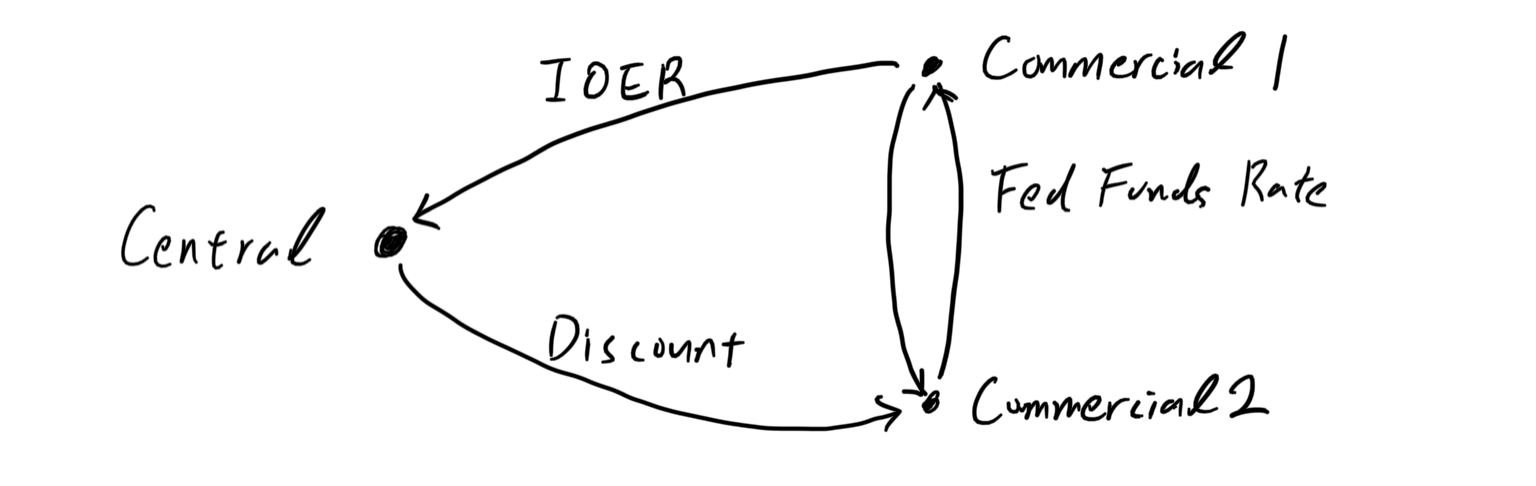
\includegraphics[scale=0.25]{img/Central_Commercial_Bank_Graph.PNG}
      \end{center}
      The IOER is the interest on the flow of money from commercial banks to the central bank. The discount rate is the interest on the flow of money from the central bank to commercial banks. The fed funds rate is the interest on the flow of money between commercial banks. 

      \begin{definition}[Open Market Operation]
        The Fed can indirectly change the actual FFR to the target rate through \textbf{open market operations (OMO)}, which are the purchases and sales of primarily U.S. Treasury securities (bonds) on the open market (and sometimes commercial securities) in order to regulate the supply of money that is on reserve in U.S. banks. In the simplest sense, 
        \begin{enumerate}
          \item If the Fed wants the FFR to decrease, then it buys government securities (with possibly newly printed money) from a group of banks. As a result, those banks end up holding fewer securities and more excess cash reserves, which they then lend out in the federal funds market to other banks. This increase in the supply of available reserves causes the federal funds rate to decrease. 
          \item If the Fed wants the FFR to increase, it does the reverse open market operation of selling government securities to the banks, taking money out of circulation and making loans harder to obtain due to a decreased supply of available reserves. This causes the federal funds rate to rise. 
        \end{enumerate}
        As shown before, the federal funds rate may increase or decrease depending on the overall supply of reserves in the federal funds market. If the supply increases, this surplus of reserves pulls the FFR down, and if the supply decreases, this shortage of reserves pushes the FFR up; therefore, the federal funds rate acts as a catalyst that brings the federal funds market to equilibrium, ensuring that supply satisfies demand with the proper interest rate. 

        We can also categories OMOs as such: 
        \begin{enumerate}
            \item \textbf{Permanent Open Market Operations (POMOs)} refers to when the central bank actively buys and sells treasury securities in the open market on a continual basis. When any central bank \textit{consistently} uses the open market to buy/sell securities in order to adjust the money supply, it is engaging in POMOs. 
            \item \textbf{Temporary Open Market Operations} refers to when specific quantities of treasury securities are authorized to be purchased or sold for a period to address a financial crisis or other economic emergency. This is used to add or drain reserves available to the banking system on a temporary basis. 
        \end{enumerate}
      \end{definition}

      \begin{example}
        We list some of the rates from May 2015 to now, with gaps of a few months in between (even though the rates change every month). 
        \begin{center}
        \begin{tabular}{r|l|l|l}
          Date & FFR& IOER & Discount Rate\\
          \hline
          05/01/2015 & 0.12\% & 0.25\% & 1\% \\
          11/01/2015 & 0.12\% & 0.25\% & 1\% \\
          12/01/2015 & 0.24\% & 0.37\% & 1\% \\
          02/01/2016 & 0.38\% & 0.5\% & 1\% \\
          10/01/2016 & 0.4\% & 0.5\% & 1\% \\
          01/01/2017 & 0.65\% & 0.75\% & 1\% \\
          04/01/2017 & 0.9\% & 1\% & 1.5\% \\
          08/01/2017 & 1.16\% & 1.25\% & 1.75\% \\
          01/01/2018 & 1.41\% & 1.5\% & 2\% \\
          04/01/2018 & 1.68\% & 1.75\% & 2.25\% \\
          08/01/2018 & 1.91\% & 1.95\% & 2.5\% \\
          10/01/2018 & 2.19\% & 2.2\% & 2.75\% \\
          03/01/2019 & 2.41\% & 2.4\% & 3\% \\
          07/01/2019 & 2.4\% & 2.35\% & 3\% \\
          11/01/2019 & 1.55\% & 1.55\% & 2.25\% \\
          04/01/2020 & 0.05\% & 0.1\% & 0.25\% 
        \end{tabular}
        \end{center}
      \end{example}

      From looking at the data, all of these interest rates tend to rise and fall together, and usually
      \[\text{FFR} < \text{IOER} < \text{Discount Rate}\]
      This makes sense because the Fed would encourage commercial banks to borrow from each other rather than hold excess reserves, which is preferred over borrowing money directly from the Fed. But in extreme situations, the above inequality may not hold for brief periods. 

    \subsubsection{Fractional Reserve Banking and the Money Multiplier}

      \begin{definition}[The Credit Market Funnel]
        Suppose the U.S. Treasury prints \$10 billion in new bills, and the Fed credits an additional \$90 billion in readily liquifiable accounts. At first, it might seem like the economy just received a monetary influx of \$100 billion, but that is actually a very small percentage of the actual money creation. 

        Nearly all of that \$100 billion enters banking reserves, but with the legally required reserve ratio of 10\%, the new \$100 billion in bank reserves could potentially result in a nominal monetary increase of \$1 trillion. 
      \end{definition}

      \begin{definition}[Money Multiplier Effect]
        When the central bank creates monetary reserves and sends those to commercial banks, banks can lend much of that money to consumers, who will also deposit most into other banks. 
      \end{definition}

      \begin{example}
        For example, if the Fed issues \$1 billion in reserves to a bank, the bank can then lend \$900 million to borrowers. These borrowers will then ultimately deposit those funds back to the banking systems (either directly or indirectly from people paid with the loaned money), which can then be loaned out at 90\%—so if that \$900 million is deposited, an additional \$810 million may be deposited. Ultimately, through this money multiplier effect, the \$1 billion in reserves will turn into \$10 billion in new credit money in the economy.
      \end{example}

    \subsubsection{Monetary Policy}

      Setting borrowing costs is how the Fed does its job; steering the world's largest economy between recession and overheating. They determine how "hot" the economy is by looking at various measures. The two most important ones are: 
      \begin{enumerate}
        \item Inflation, measured by the CPI/PPI, and usually targeted to be at 2\%. 
        \item Unemployment rate, measured by the CPS, which should be minimized. 
      \end{enumerate}
      We have already seen how the Fed uses open market operations to adjust the FFR. But how does this exactly affect other rates? In the simplest terms, 
      \begin{enumerate}
        \item A decreased FFR means that banks can borrow money easily at low interest rates, meaning that they can then use the reserves that they have obtained at lower rates to offer loans at lower interest rates to consumers/businesses. The cheaper credit in turn causes consumers/businesses to spend and invest, boosting sales and economic activity (an \textbf{expansionary goal}). 
        
        Furthermore, an decreased FFR, which implies lower yields, tend to push away investment capital from investors abroad seeking higher returns on bonds and interest-rate products. This makes the U.S. dollar weaker. 
        
        \item An increased FFR means that banks borrow less money due to higher interest rates, meaning that they give loans at even higher ones to consumers. This increase in the cost of credit through the funds rate curbs demand and reduces consumers/firms taking out loans to spend and invest, leading to an economic cooldown (a \textbf{contractionary goal}). 
        
        Furthermore, an increased FFR, which implies higher yields, tend to attract investment capital from investors abroad seeking higher returns on bonds and interest-rate products. This makes the U.S. dollar stronger. 
      \end{enumerate}

      Note that the FFR is the \textit{benchmark interest rate} of the economy, since all other interest rates on loans from commercial banks are dependent on it. That is, a higher FFR will mean that commercial banks will have to raise interest rates on all of their loans (to profit accordingly), and a lower FFR will mean that banks will lower their interest rates on loans. Therefore consumers should care about the FFR since it influences how much they pay to borrow and how much they're paid to save. 

      Let's talk about what aspects of the economy the FFR affects: 
      \begin{enumerate}
        \item Bond market. Remember that when interest rates rise, bond prices generally fall (in the secondary market), and when interest rates fall, bond prices generally rise. However, in the primary market, how does the original coupon rate get established? 
        
        \item \textbf{Prime Rates}, or the \textbf{Bank Prime Loan Rate}, is the credit rate that banks extend to their most credit-worthy customers, leading to a rise in every other interest rate. Since the FFR determines the minimum interest rate that banks must put on a loan to make a profit, it is clear that 
        \[\text{Increased Fed funds rate } \implies \text{ Increased prime rate}\]
        In fact, prime rates are pegged at 300 points (3\%) over the target rate. Since prime rates represent the base rate at which banks loan out to consumers, an increase in this base rate will increase every other rate, such as 
        \begin{enumerate}
            \item Adjustable-rate mortgages
            \item Auto loans
            \item Variable-rate credit card expenses
            \item CDs, savings accounts, and money market accounts
        \end{enumerate}
        depending on factors such as one's assets, liabilities, and creditworthiness. 
        \item If global capital flows are moving into dollar-denominated assets, chasing higher rates of return, the U.S. dollar strengthens, causing it to be more expensive in the exchange rate. 
        \item \textbf{Exports}: Due to the dollar strength, U.S. export sales may decline since foreign countries will need to pay more for U.S. goods. 
        \item \textbf{Imports, Inflation:} A strong dollar makes foreign imports cheaper, since the price of foreign currency is relatively cheap. This results in cheaper products at U.S. stores (since domestic companies have to keep prices low to compete with cheap foreign imports), and these low prices translate to low inflation. 
      \end{enumerate}
      On the extreme end, zero and negative rate environments benefit the economy through easier borrowing. In an extreme negative rate environment, borrowers even receive interest payments. 

      \begin{definition}[Other Monetary Policy Tools]
        Most of the time, the Fed funds rate is unchanged or changed incrementally by 0.25\%, but in extreme cases, the rate can change drastically. However, in less extreme cases, the Fed can also adjust these rates too to influence monetary policy. 
        \begin{enumerate}
          \item \textit{It can change the bank reserve requirements.} If they are higher, more money is "locked in" the required reserve and the money supply shrinks. If they are lower, more money moves from the required reserve to the excess reserve, allowing better trading rates. 
          \item \textit{It can change the discount rates.} If the discount rates are higher, it will discourage commercial banks from loaning money from the Fed, and if rates are lower, commercial banks have more of an incentive to loan money from central banks. 
          \item \textit{It can change the IOR/IOER}. If the IOER rate is low, banks would prefer to lend funds out since it will be more profitable to gain interest according to the FFR rather than the IOER. This increases cash circulation and makes it easier to borrow money. If the IOER rate is high, then banks would prefer to keep more money at the Fed rather than lend to a potentially risky borrower. This chokes the circulation of money since banks won't want to take money out of their excess reserves. 
        \end{enumerate}
      \end{definition}

  \subsection{Gross Domestic Product}

    \begin{definition}[Gross Domestic Product]
      If we think of a nation as a giant firm that takes in inputs and produces outputs, then the \textbf{gross domestic product (GDP)} is the total monetary or market value of all the finished goods and services produced within a country's borders in a specific time period. As a broad measure of overall domestic production, it functions as a comprehensive scorecard of a given country's economic health within the international market. It is typically calculated on an annual basis (\textit{annualized GDP}), and sometimes on a quarterly one. There are multiple ways we can measure GDP: 
      \begin{enumerate}
        \item \textbf{Nominal GDP} does not take into account inflation. It is an assessment of economic production in terms of the current prices of goods and services.  
        \item \textbf{Real GDP} does take inflation into account, allowing it to be measured in current dollars. 
        \item \textbf{GDP Growth} compares the year-over-year change in a country's economic output in order to measure how fast an economy is growing, expressed as a percentage rate. If GDP growth rates accelerate, it may be a signal that the economy is "overheating" and the central bank may seek to raise interest rates. Conversely, a shrinking (or negative) GDP growth rate is a signal that rates should be lowered and that stimulus may be necessary. 
        \item \textbf{GDP Purchasing Power Parity (PPP)} is a method to see how one country's GDP measures up in "international dollars" using a method that adjusts for differences in local prices and costs of living in order to make cross-country comparisons. 
        \item \textbf{GDP per capita} is a measurement of the GDP per person in a country's population. It indicates the amount of output or income per person in an economy and can indicate average productivity or average living standards. GDP per capita can be stated in nominal, real, or PPP terms. 
      \end{enumerate}
    \end{definition}

    There are three ways of calculating the GDP of a nation, all of which should theoretically add to the same value. 
    \begin{enumerate}
        \item Production Approach
        \item Income Approach
        \item Expenditure Approach
    \end{enumerate}

    \begin{definition}[Expenditure Approach]
    The \textbf{expenditure/spending approach} calculates spending by the different groups that participate in the economy. It can be calculated using the following formula: 
    \[GDP = C + G + I + NX\]
    where
    \begin{enumerate}
        \item $C = $ Consumption; This refers to private consumption expenditures or consumer spending. Consumers spend money to acquire goods and services, such as groceries and haircuts (which are goods and services produced). Consumer spending is the biggest component of GDP, accounting for more then $2/3$ of the U.S. GDP. Consumer confidence, therefore, has a very significant bearing on economic growth. 
        \item $G = $ Government Spending; This represents government consumption expenditure and gross investment. For example, governments spend money on equipment, infrastructure, and payroll. 
        \item $I = $ Investment; This refers to private domestic investment or capital expenditures (i.e. company expenditures). Businesses spend money in order to invest in their business activities, such as buying machinery. 
        \item $NX = $ Net exports (which is Exports$-$Imports) All expenditures by companies located in a given country, even if they are foreign companies, are included in this calculation. 
    \end{enumerate}
    \end{definition}

    There is another important economic measurement of a country. 

    \begin{definition}[Gross National Income]
    The difference between GDP and \textbf{Gross National Income (GNI)} is that GDP defines its scope according to location, while GNI defines its scope according to ownership. That is, GNI is product produced by enterprises owned by a country's citizens, even in foreign countries.

    It is clear to see by definition 
    \begin{align*}
        GNI = GDP & + (\text{income receipts from the rest of the world}) \\
        & - (\text{income payments from the rest of the world})
    \end{align*}
    \end{definition}

\end{document}
